\begin{frame}
	\frametitle{\subsecname}
	Aquí es conveniente representar cualquier sucesión de números reales $(a_{n})_{n} $ como la función $f\colon\mathds{N}\rightarrow\mathds{R}$ definido por: \[ f(n)=a_{n},\quad\forall n\in\mathds{N}. \]
	\begin{definition}
		Una \textbf{ecuación en diferencias} es una expresión de la forma:
		\begin{equation}\label{eq:diffeq}
		G\left(n,f(n),f\left(n+1\right),\ldots,f\left(n+k\right)\right)=0,\quad\forall n\in\mathds{N}.
		\end{equation}
	\end{definition}
	El \textbf{orden} de una ecuación en diferencias se halla mediante la diferencia entre los ``términos mayor'' y ``menor'' respectivamente. En~(2), es \alert{$n+k-n=k$}.%\eqref{eq:diffeq}
	\begin{example}
		\begin{itemize}
			\item El \alert{orden} de $f\left(n+3\right)-f\left(n+1\right)-5f(n)=n$ es \alert{$3$}.
			\item El \alert{orden} de $f\left(n+3\right)-f\left(n+1\right)=n^{2}-3$ es \alert{$2$}.
		\end{itemize}
	\end{example}
\end{frame}

\begin{frame}
	\begin{definition}
		La \textbf{solución} de~(2) a toda sucesión $\{f\left(0\right),f\left(1\right),\ldots,f(n),\ldots\}$ que la satisfaga, ahora se le llama \emph{solución general} de una E.D al conjunto de todas las soluciones que tendrán tanto parámetros como orden tenga la ecuación. La determinación de estos parámetros, a partir de unas condiciones iniciales, nos proporcionará las distintas soluciones particulares.
	\end{definition}

	\begin{example}
		Sea \[ f\left(n+1\right)-f\left(n\right)=3 \] una ecuación en diferencias de orden uno cuya solución general es $f\left(n\right)=3n+c$.

	\

		Si consideramos las condiciones iniciales, por ejemplo, $f(0)=2$, entonces $f(0)=3\times0+c=c$, por tanto $c=2$ y la solución particular es $f_{p}(n)=3n+2$.
		Es decir, la solución es la sucesión $f_{p}(n)=\left\{2,5,8,11,\ldots\right\}$.
	\end{example}
\end{frame}

\begin{frame}
	\begin{definition}
		Llamamos ecuación en diferencias lineal de orden $k$ a toda expresión de la forma:
		\[ f\left(n+k\right)+a_{1}(n)f\left(n+k-1\right)+\cdots+a_{k-1}(n)f\left(n+1\right)+a_{k}(n)f\left(n\right)=b\left(n\right), \]
		donde $a_{k}(n)\neq0$.
	\end{definition}

	\begin{block}{Clasificación de las ecuaciones de diferencias lineal}
		\begin{itemize}
			\item Homogéneas si $b(n)=0$.
			\item Completas si $b(n)\neq0$.
			\item De coeficientes constantes si $a_{i}(n)=a_{i}$, $\forall i$.
			\item De coeficientes no constantes si $a_{i}(n)\neq a_{i}$ para algún $i$.
		\end{itemize}
	\end{block}
\end{frame}

\begin{frame}
	\begin{theorem}[De la existencia y la unicidad]
		Dada la ecuación: \[ f\left(n+k\right)+a_{1}(n)f\left(n+k-1\right)+\cdots+a_{n-1}(n)f\left(n+1\right)+a_{n}(n)f\left(n\right)=0, \] y dados $n$ números reales $k_{0}$, $k_{1}$, \ldots, $k_{n-1}$ existe una única solución que verifica \[ f\left(0\right)=k_{0},f\left(1\right)=k_{1},\ldots,f\left(n-1\right)=k_{n-1}. \]
	\end{theorem}

	\begin{theorem}
		Toda combinación lineal de soluciones de una ecuación en diferencias lineal homogénea de orden $n$ es también una solución.
	\end{theorem}

	\begin{corollary}
		Las soluciones de una ecuación en diferencia lineal de orden $n$ forman un espacio vectorial.
	\end{corollary}

	\begin{theorem}
		La dimensión del espacio de soluciones de una ecuación en diferencias lineal de orden $n$ es $n$.
	\end{theorem}
\end{frame}

%http://personal.us.es/pnadal/Informacion/leccion5ecdiferencias.pdf
%\begin{frame}
%	\begin{block}{Ecuaciones en diferencias de primer orden}
%	\end{block}
%	
%	\begin{block}{Ecuaciones en diferencias de segundo orden}
%	\end{block}
%\end{frame}

\subsubsection{Número de Catalan}

\begin{frame}{Número de Catalan}
	\begin{block}{Triangulación}
		\begin{figure}
			\centering
			
\includegraphics[height=0.3\paperheight]{ca1}
		\end{figure}
	\end{block}
	
	\begin{block}{Caminos monótonos}
		\begin{figure}
			\centering
			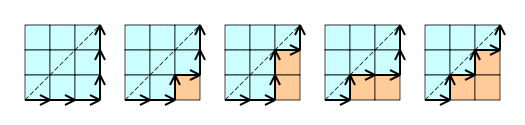
\includegraphics[height=0.3\paperheight]{ca2}
		\end{figure}
	\end{block}
\end{frame}